\section{EBSD Data Analysis}

\begin{frame}[fragile]
  \frametitle{Single Orientation Meassurments - The class EBSD}

  Data stored in the class \alert{EBSD}

  \medskip

  \begin{columns}


    \begin{column}{6cm}

      basic characteristics:
      \begin{itemize}
      \item crystal symmetry
      \item specimen symmetry
      \item single orientations
      \item phase information
      \end{itemize}

    \end{column}

    \begin{column}{5.5cm}

      additional properties:
      \begin{itemize}
      \item spatial coordinates
      \item Error
      \item IQ, CI, FIT
      \item ...
      \end{itemize}
    \end{column}
  \end{columns}

  \bigskip

  \begin{columns}
    \begin{column}{8cm}
      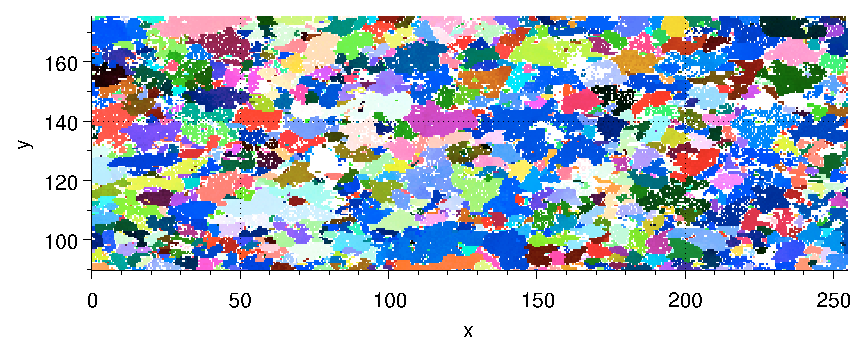
\includegraphics[height=3.5cm]{pic/ebsd.pdf}
    \end{column}
    \begin{column}{4cm}
      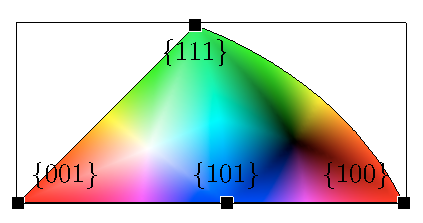
\includegraphics[width=4cm]{pic/ebsdtriangle.pdf}
    \end{column}
  \end{columns}
\end{frame}

\subsection*{Importing EBSD Data}
\begin{frame}[fragile]
  \frametitle{Importing EBSD Data - The Import Wizard}

  \begin{columns}

    \begin{column}{6cm}
      Formats supported by \MTEX:
      \begin{itemize}
      \item HKL: *.ang
      \item Channel: *.ctf
      \item generic: *.txt, *.xls
      \end{itemize}

    \end{column}

    \onslide<1->

    \begin{column}{6cm}
      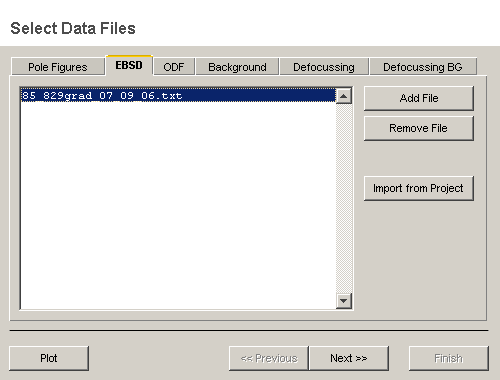
\includegraphics[width=6cm]{pic/iw2}
    \end{column}

  \end{columns}

\end{frame}


\begin{frame}[fragile]
  \frametitle{Importing EBSD Data - Using a Script}

Script generated by the import wizard:

\begin{lstlisting}
CS = { symmetry('m-3m'), ...
       symmetry('m-3m') }
SS = symmetry('triclinic');
\end{lstlisting}

\begin{lstlisting}
fname = { [ pathto '85_829grad_07_09_06.txt']};
\end{lstlisting}

\begin{actionenv}<1-| alert@1->
\begin{lstlisting}
	ebsd = loadEBSD(fname,CS,SS,'interface',interf,...
	  'ColumnNames', {'Phase' 'x' 'y' ...},...
	  'Columns', [2 3 4 ...],'Bunge',...
	  'ignorePhase', 0);
\end{lstlisting}
\end{actionenv}

\end{frame}

\subsection*{Visualization}

\begin{frame}[fragile]
  \frametitle{Visualize EBSD Data in \MTEX}

  \begin{columns}
    \begin{column}{8.5cm}

Scatter plots in Rodriguez space or axis angle space

\begin{lstlisting}
		scatter(ebsd)
\end{lstlisting}

\pause

Scatter plots in pole figures, inverse pole figures, or ODF sections


\begin{onlyenv}<1,3- |handout:1>
\begin{lstlisting}
		plotpdf(ebsd,[Miller(0,0,1),...])
		plotipdf(ebsd,vector3d(1,0,0))
		plotodf(ebsd)
\end{lstlisting}
\end{onlyenv}

\begin{onlyenv}<2 |handout:0>
\begin{lstlisting}
		/+plotpdf(ebsd,[Miller(0,0,1),...])+/
		plotipdf(ebsd,vector3d(1,0,0))
		plotodf(ebsd)
\end{lstlisting}
\end{onlyenv}

\pause

Spatial plots of EBSD data

\begin{onlyenv}<1-2|handout:0>
\begin{lstlisting}
plot(ebsd)
plot(ebsd,'colorcoding','ipdf')
plot(ebsd,'property','phase')
plot(ebsd,'property','mad')
\end{lstlisting}
\end{onlyenv}

\begin{onlyenv}<3 |handout:1>
\begin{lstlisting}
/+plot(ebsd)+/
/+plot(ebsd,'colorcoding','ipdf')+/
plot(ebsd,'property','phase')
plot(ebsd,'property','mad')
\end{lstlisting}
\end{onlyenv}

\begin{onlyenv}<4 |handout:0>
\begin{lstlisting}
plot(ebsd)
plot(ebsd,'colorcoding','ipdf')
/+plot(ebsd,'property','phase')+/
plot(ebsd,'property','mad')
\end{lstlisting}
\end{onlyenv}

\begin{onlyenv}<5 |handout:0>
\begin{lstlisting}
plot(ebsd)
plot(ebsd,'colorcoding','ipdf')
plot(ebsd,'property','phase')
/+plot(ebsd,'property','mad')+/
\end{lstlisting}
\end{onlyenv}

      Color-Codings: ipdf, bunge, ihs, angle, sigma

    \end{column}

    \begin{column}{3.5cm}
      \only<1 |handout:0>{%
      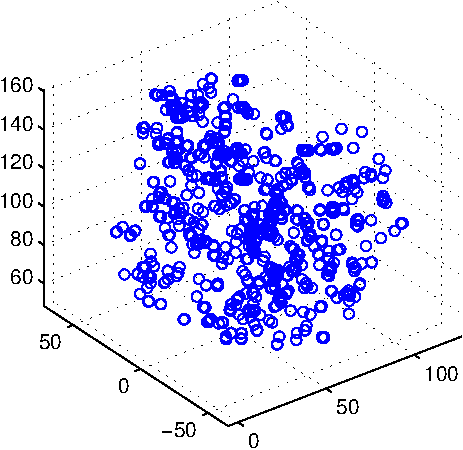
\includegraphics[width=3.5cm]{pic/ebsdscatter}%
      }%
      \only<2|handout:0>{%
      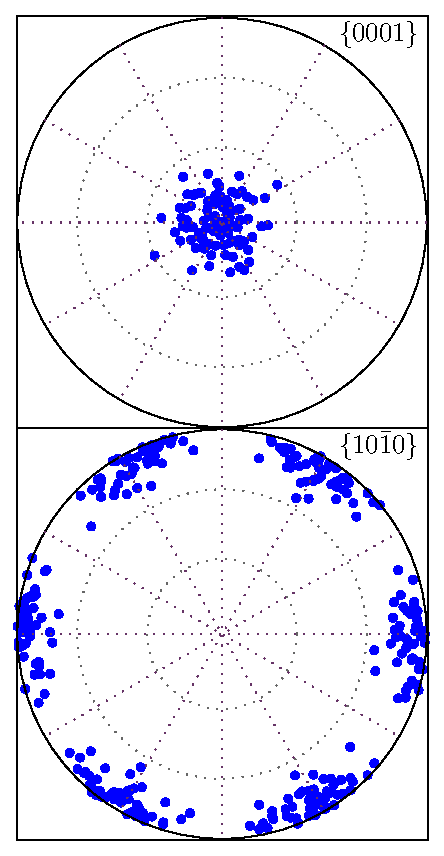
\includegraphics[width=3.2cm]{pic/EBSDpdf}%
      }%
      \only<3|handout:1>{%
      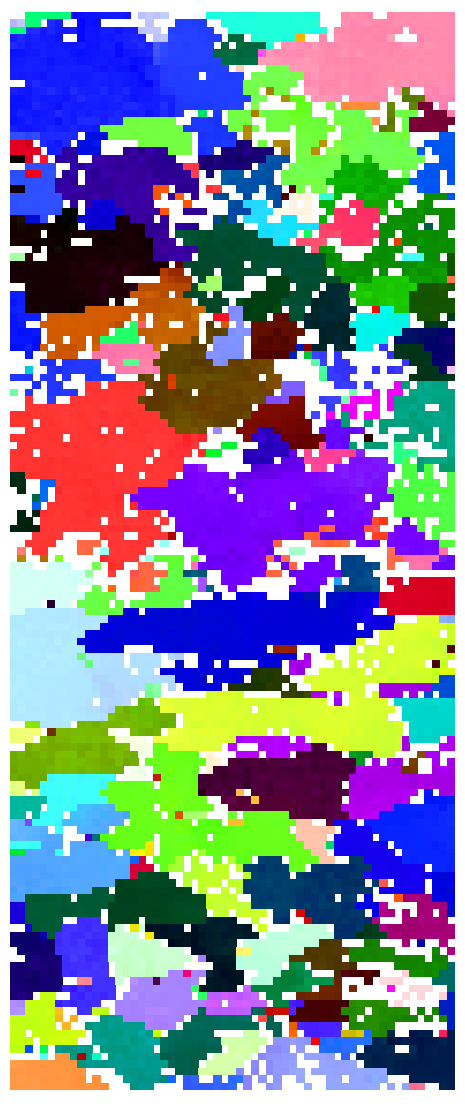
\includegraphics[height=7.5cm]{pic/ebsdsmall}%
      }%
      \only<4|handout:0>{%
      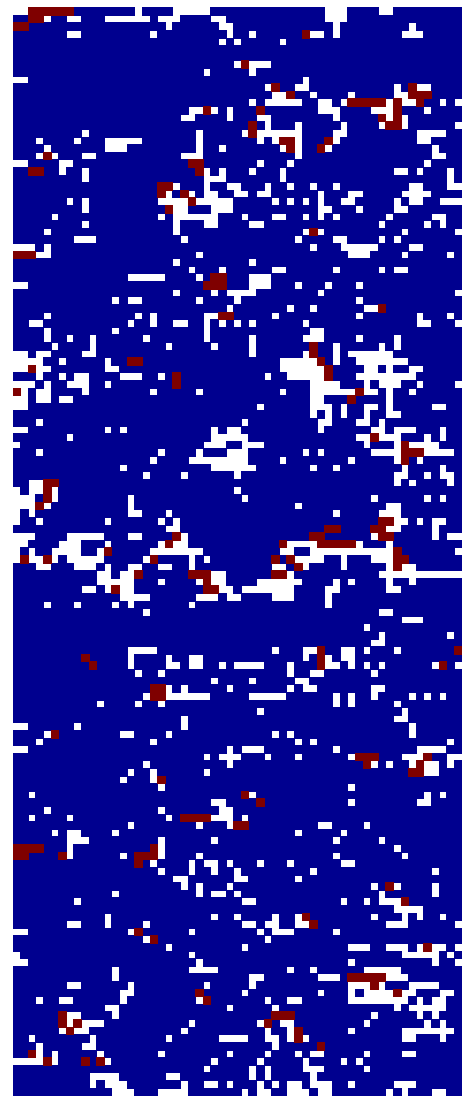
\includegraphics[height=7.5cm]{pic/ebsdphase}%
      }%
      \only<5|handout:0>{%
      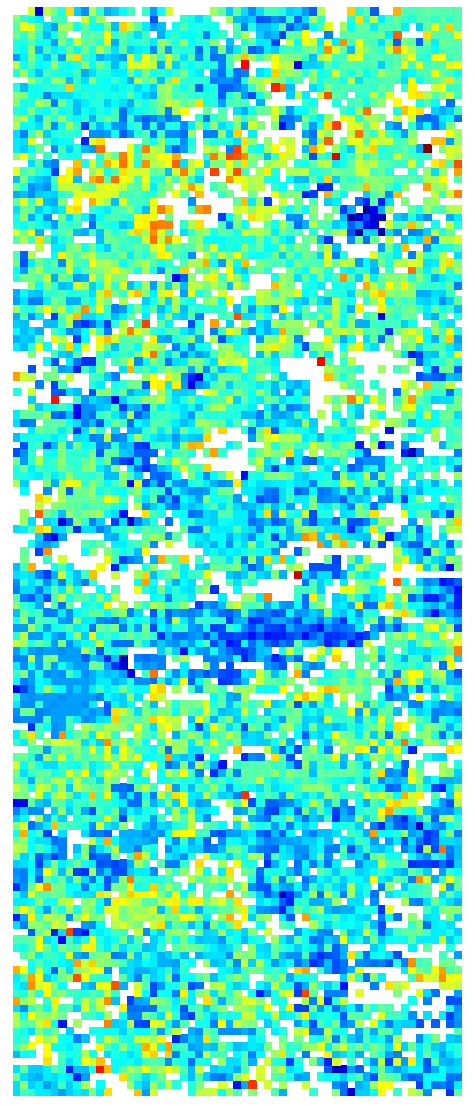
\includegraphics[height=7.5cm]{pic/ebsdmad}%
      }%
    \end{column}
  \end{columns}
\end{frame}

\subsection*{Grains Analysis}

\begin{frame}[fragile]
  \frametitle{Grain Analysis with \mtex}



  \begin{columns}
    \begin{column}{8.5cm}

      A grain is defined as a region in which the mis\-orien\-tation of
      at least one neigh\-bour\-ing meas\-ure\-ment-site is lower than a choosen threshold

\medskip

      Grain Detection

\begin{lstlisting}
[grains ebsd] = segment2d(ebsd,...)
\end{lstlisting}

      \medskip
      Options:
\begin{lstlisting}
'angle'        % threshold angle
'distance'     % max distance
'augmentation' % bounding box
'unitcell'     % no voronoi
\end{lstlisting}

\medskip

Plot grain boundaries:
\begin{lstlisting}
hold on, plot(grains,'color','k')
\end{lstlisting}

\end{column}
    \begin{column}{3.5cm}
      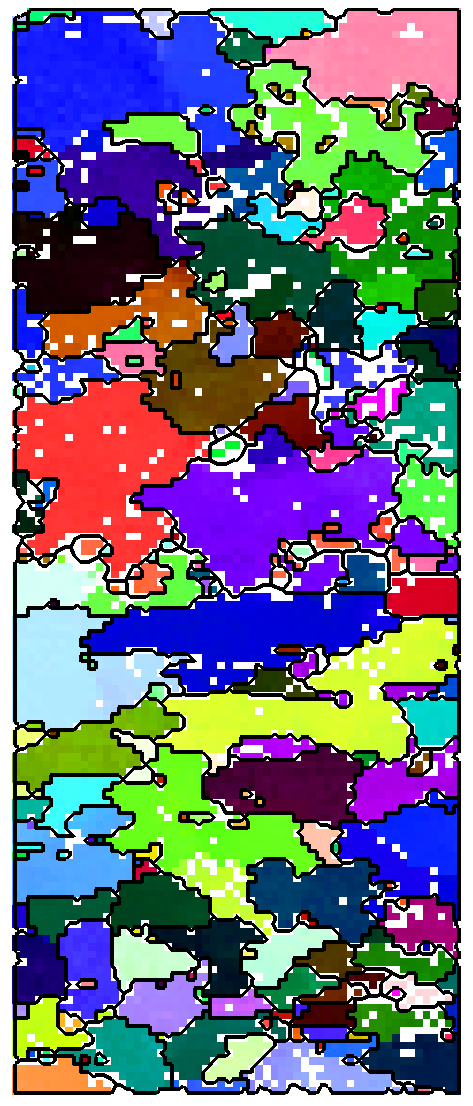
\includegraphics[height=7.5cm]{pic/ebsdgrains}
    \end{column}
  \end{columns}

\end{frame}


\begin{frame}[fragile]
  \frametitle{Grain Properties}

  \begin{columns}
    \begin{column}{8.5cm}


      Copy EBSD properties to the grains

\begin{onlyenv}<1 |handout:1>
\begin{lstlisting}
grains = copyproperty(grains,ebsd)

/+plot(grains,'property','orientation')+/
plot(grains,'property',phase')
\end{lstlisting}
\end{onlyenv}

\begin{onlyenv}<2- |handout:0>
\begin{lstlisting}
grains = copyproperty(grains,ebsd)

plot(grains,'property','orientation')
/+plot(grains,'property',phase')+/
\end{lstlisting}
\end{onlyenv}

\pause
\pause

Access to Properties
\begin{lstlisting}
phase   = get(grains,'phase')
grains1 = grains(phase == 1)
orient  = get(grains,'orientation')
\end{lstlisting}

Interconnection with EBSD Data
\begin{lstlisting}
[grains ebsd] = link(grains,ebsd)
[ebsd grains] = link(ebsd,grains)
\end{lstlisting}

    \end{column}
    \begin{column}{3.5cm}
      \only<1|handout:1>{%
      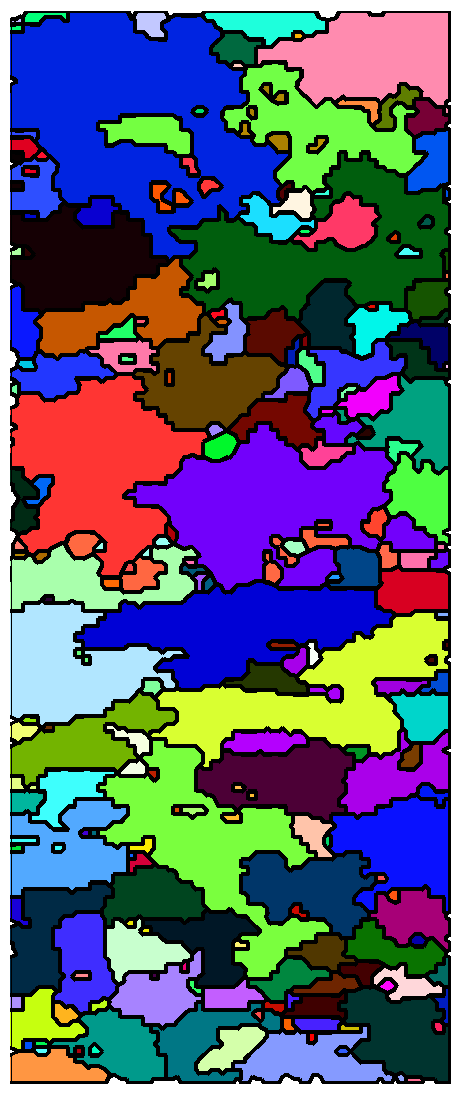
\includegraphics[height=7.5cm]{pic/ebsdgrainorientation}%
      }%
      \only<2-|handout:0>{%
      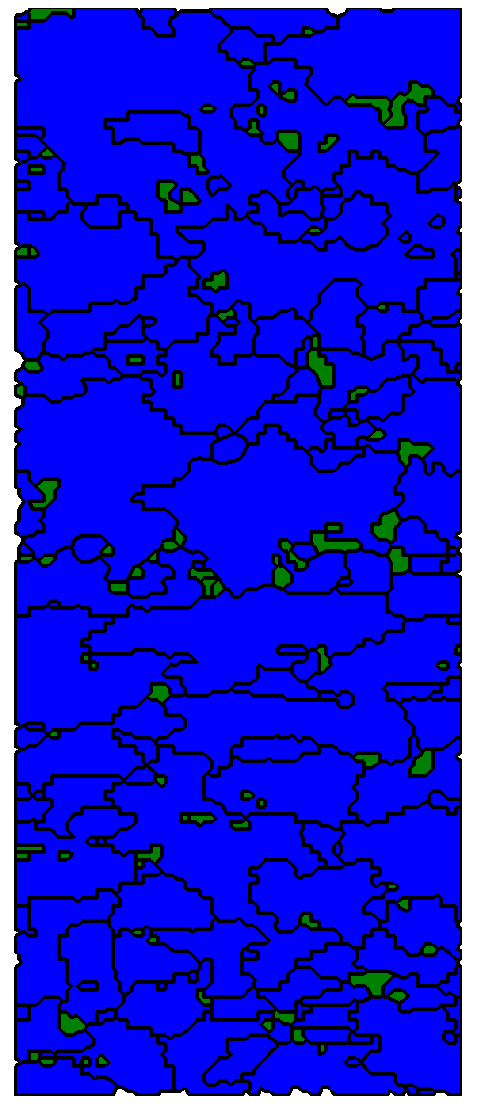
\includegraphics[height=7.5cm]{pic/ebsdgrainsphase}%
      }%
    \end{column}
  \end{columns}

\end{frame}


%
\begin{frame}[fragile]
  \frametitle{Grain Properties: Geometry}

Basic functions on grain geometry
\begin{lstlisting}[basicstyle=\footnotesize]
area,perimeter,centroid,hullarea,hullperimeter,
hullcentroid,aspectratio,shapefactor,borderlength,
deltaarea,equivalentperimeter,grainsize,paris
\end{lstlisting}
%

\begin{columns}[t]
  \begin{column}[T]{6.5cm}
  Grain-Size distribution
\begin{lstlisting}
A = area(grains);
% histogram
bar( hist(A,exp(-1.5:6.5)) )
\end{lstlisting}

Other Properties:
\begin{lstlisting}[basicstyle=\footnotesize]
hasholes,hassubfraction
\end{lstlisting}

	\end{column}
	\begin{column}[T]{5cm}
		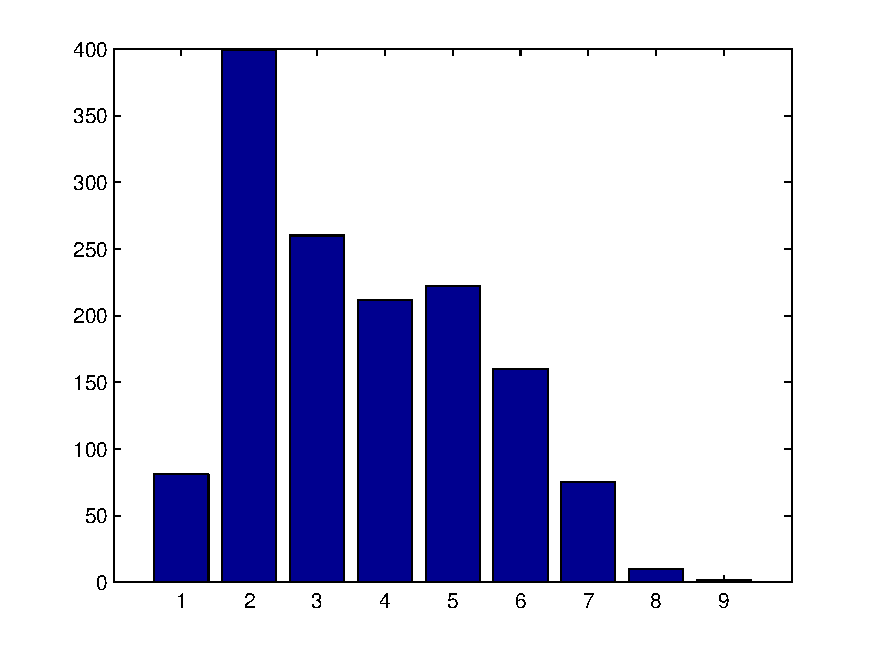
\includegraphics[width=5cm]{pic/grh}
	\end{column}
\end{columns}

Selecting grains after properties
\begin{lstlisting}
grains = grains( area(grains) > mean(area(grains)) )
\end{lstlisting}

\end{frame}


%
\begin{frame}[fragile]
  \frametitle{Working with EBSD Data Directly}

	Access EBSD Properties
\begin{lstlisting}
	orientations = get(ebsd,'orientation')
	x = get(ebsd,'x')
\end{lstlisting}

	\medskip

	Rotate EBSD Data
\begin{lstlisting}
	rot = axis2quat(xvector,90*degree)
	ebsd = rotate(ebsd,rot)
\end{lstlisting}

	\medskip
        Omit one pixel grains
\begin{lstlisting}
%grains containing more than one pixel
grains = grains(grainsize(grains) > 1)

%restrict ebsd data to those grains
ebsd = link(ebsd,grains)
\end{lstlisting}

\end{frame}

\subsection*{EBSD - to - ODF Reconstruction}


\begin{frame}[fragile]
  \frametitle{EBSD to ODF Reconstruction in \MTEX}

  \mtex uses kernel density estimation to compute an ODF from EBSD data. The
  sensitive parameter of this method is the kernel function.

\medskip

  Syntax:
  \begin{alertenv}
\begin{lstlisting}
odf = calcODF(ebsd,<options>)
\end{lstlisting}
  \end{alertenv}

Options:
\lstset{emph={bandwidth},emphstyle={}}
\begin{lstlisting}
'kernel'     % the kernel to be used
'halfwidth'  % halfwidth of the kernel function
'resolution' % resolution of the approximation grid

'Fourier'    % ODF by its Fourier coefficients
'exact'      % no approximation to a corser grid
\end{lstlisting}


\end{frame}

%\subsection*{EBSD Simulation}

\begin{frame}[fragile]
  \frametitle{EBSD Simulation in \mtex}

  Simulation of EBSD data may help to analyze the error made by ODF kernel
  density estimation from real data.

\begin{lstlisting}
ebsd = simulateEBSD(santafee,5000)
\end{lstlisting}

Compute the error between the original ODF and the estimated ODF.
\begin{lstlisting}
error = calcerror(santafee,calcODF(ebsd))
\end{lstlisting}

      \centerline{
      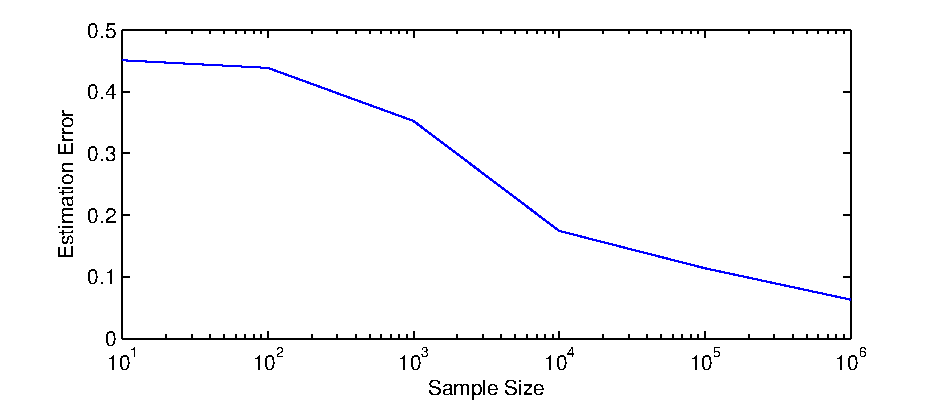
\includegraphics[width=10cm]{pic/ebsdcorrectness}}

\end{frame}





\begin{frame}[fragile]
  \frametitle{ODF Estimation of Grains: Macrotexture}


\begin{columns}[t]
\begin{column}[T]{8cm}

Estimation on Mean Orientation

\begin{lstlisting}
grains = mean(grains,ebsd)
grains = calcODF(grains,...)
\end{lstlisting}

\medskip

Options already known from previous
\begin{lstlisting}[basicstyle=\footnotesize]
'kernel', 'halfwidth', 'resolution'
\end{lstlisting}

\medskip

Compare it with original EBSD Data
\begin{onlyenv}<1|handout:0>
\begin{lstlisting}
/+odf1 = calcODF(ebsd,...)+/
odf2 = calcODF(grains,...)
calcerror(odf1,odf2)
\end{lstlisting}
\end{onlyenv}

\begin{onlyenv}<2|handout:1>
\begin{lstlisting}
odf1 = calcODF(ebsd,...)
/+odf2 = calcODF(grains,...)+/
calcerror(odf1,odf2)
\end{lstlisting}
\end{onlyenv}

\end{column}
\begin{column}[T]{3.5cm}
\only<1 | handout:0>{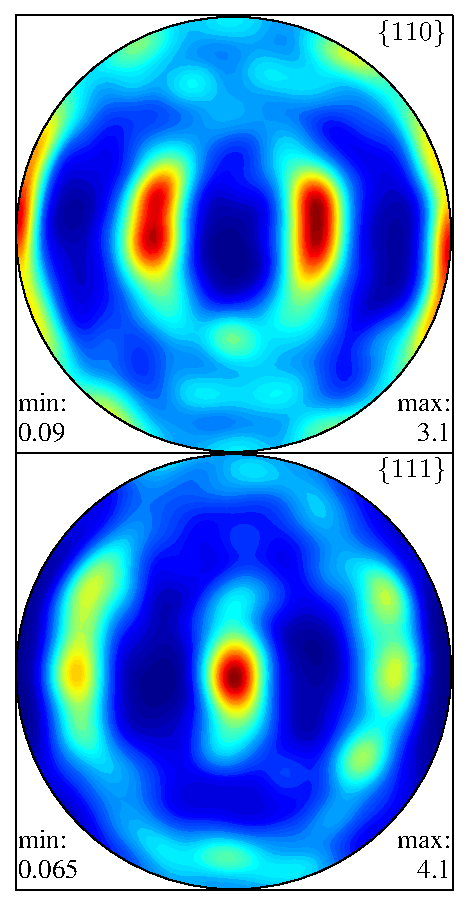
\includegraphics[width=3.5cm]{pic/odf_gr_e}}
\only<2 | handout:1>{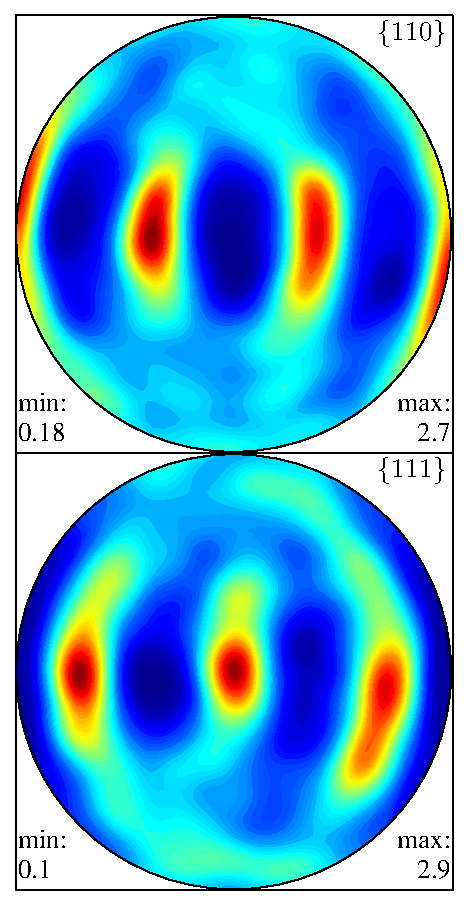
\includegraphics[width=3.5cm]{pic/odf_gr_g}}
\end{column}
\end{columns}

\end{frame}


\begin{frame}[fragile]
  \frametitle{ODF Estimation of Grains: Microtexture}

Estimation of individual Grain-ODFs on underlaying EBSD Data
\begin{lstlisting}
grains = calcODF(grains,ebsd, ...)
grains = calcODF(grains,ebsd_mis2mean,...
									  'property','ODF_mis',...)
\end{lstlisting}

Applying functions on grain-ODFs
\begin{lstlisting}
tindex = grainfun(function_handle,grains,'ODF',...)
tindex = grainfun(@textureindex,grains,'ODF',...)
\end{lstlisting}

\begin{columns}
\begin{column}[T]{3.5cm}
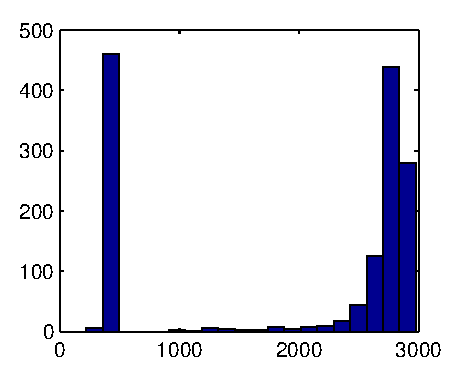
\includegraphics[width=3.5cm]{pic/grtindxhist}
\end{column}
\begin{column}[T]{8cm}
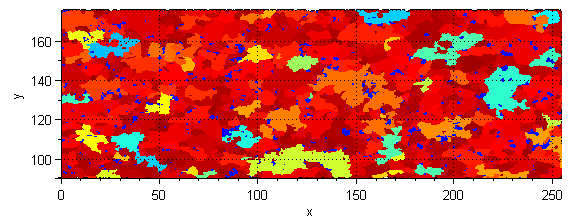
\includegraphics[width=8cm]{pic/grtindx}
\end{column}
\end{columns}

\end{frame}



\begin{frame}[fragile]
  \frametitle{Misorientation \uncover<2->{and Mesotexture}}

To treat Misorientation of every grain requires an assigned orientation
\begin{lstlisting}
grains = mean(grains,ebsd)
\end{lstlisting}

Misorientation of underlaying EBSD Data to its mean

\begin{onlyenv}<1| handout:1>
\begin{lstlisting}
/+ebsd_mis = misorientation(grains,ebsd)+/
\end{lstlisting}
\end{onlyenv}
\begin{onlyenv}<2| handout:0>
\begin{lstlisting}
ebsd_mis = misorientation(grains,ebsd)
\end{lstlisting}
\end{onlyenv}

\begin{uncoverenv}<2->
\medskip
Misorientation to neighboured grains
\begin{onlyenv}<1| handout:1>
\begin{lstlisting}
ebsd_mis = misorientation(grains)
\end{lstlisting}
\end{onlyenv}
\begin{onlyenv}<2| handout:0>
\begin{lstlisting}
/+ebsd_mis = misorientation(grains)+/
\end{lstlisting}
\end{onlyenv}

\end{uncoverenv}

%\medskip
\begin{columns}[t]
\begin{column}[T]{6.25cm}
\medskip
Misorientation Distribution
\begin{lstlisting}
hist(ebsd_mis)
\end{lstlisting}

and Density Function
\begin{lstlisting}
odf = calcODF(ebsd_mis,...)
\end{lstlisting}

\end{column}
  \begin{column}[T]{5.25cm}
\only<1|handout:1>{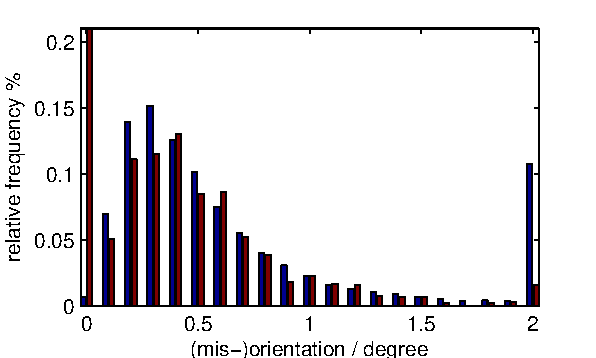
\includegraphics[height=3.5cm]{pic/mis}}
\only<2|handout:0>{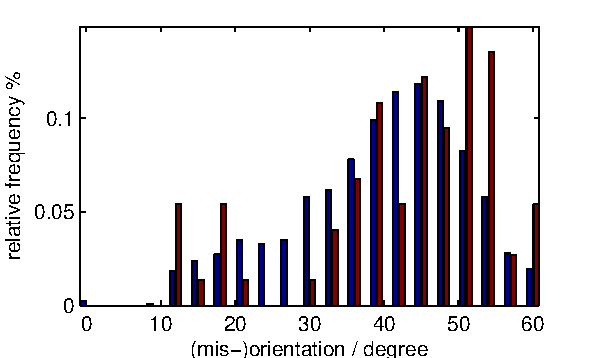
\includegraphics[height=3.5cm]{pic/mis2}}
\end{column}
\end{columns}

\end{frame}



\subsection*{Exercises}

\begin{frame}

  \begin{Exercise}
    \begin{enumerate}[a)]
    \item Load the EBSD data:
      \texttt{data/ebsd\_txt/85\_829grad\_07\_09\_06.txt}!
    \item Perform grain detection with a certain threshold!
    \item Plot the EBSD data together with the grain boundaries!
    \item Compute the mean orientation for each grain and visualize it!
    \item Compute and visualize the grains size distribution!
    \item Explore the geometric properties of the grains! Is there any
      relationship between the size and the mad of the grains?
    \end{enumerate}
  \end{Exercise}

  \begin{Exercise}
    \begin{enumerate}[a)]
    \item Estimate an ODF from the above EBSD data.
    \item Visualize the ODF and some of its pole figures!
    \item Explore the influence of the halfwidth to the kernel
      density estimation by looking at the pole figures!
    \end{enumerate}
  \end{Exercise}


\end{frame}

\begin{frame}

  % \begin{block}{Exercises 6}
  %   \begin{enumerate}
  %   \item Start with an arbitrary model ODF!
  %   \item Compute the volume portion of the ODF within a range of $20\degree$
  %     of the modalorientation and compare it to the corresponding volume of
  %     the uniform ODF!
  %   \item Simulate EBSD data from this ODF with 10.000 orientations.
  %   \item Plot pole figures from the EBSD data and compare them with the pole
  %     figures from the model ODF.
  %   \item Compute the volume portion of the estimated ODF within a range of
  %     $20\degree$ of the modalorientation and compare it to model ODF!
  %   \item Perform these investigations for different sample sizes!
  %   \end{enumerate}
  % \end{block}


  \begin{Exercise}
    \begin{enumerate}[a)]
    \item Estimate an overall grain-ODF and compare it with the ODF of
      original EBSD data
    \item Visualize the textureindex of each grain
    \item Compare the intrinsic Misorientation of individual grains to its
      texture properties, how does the threshold angle affect this?
    \item Investigate the Misorientation to neighbours, how does the threshold
      angle influence this?
    \end{enumerate}
  \end{Exercise}

\end{frame}



%%% Local Variables:
%%% mode: latex
%%% TeX-master: "main"
%%% End:
